\chapter{Implementasi dan Pengujian Perangkat Lunak}
\label{chap:Implementasi dan Pengujian Perangkat Lunak}

\section{Implementasi Perangkat Lunak}

\subsection{Lingkungan Perangkat Kerat}

Perangkat keras yang digunakan dalam membangun perangkat lunak adalah sebuah PC dengan spesifikasi berikut:

\begin{itemize}
\item \textit{Processor}: Intel i7 4790K @4.00 GHz

\item RAM: 16 GB DDR3

\item VGA: NVIDIA GeForce GTX 750TI 2GB

\item \textit{Harddisk}: 1TB + 256GB SSD 

\end{itemize}

\subsection{Lingkungan Perangkat Lunak}

Perangkat lunak yang digunakan untuk membangung perangkat lunak adalah sebagai berikut:

\begin{itemize}

\item Sistem Operasi: Ubuntu 18.04.2 LTS

\item Bahasa Pemrograman: Scala

\item IDE: InteliJ IDE 2018

\item Versi Java: JDK 1.8.0\_181

\item Versi Scala: Scala 2.11.12

\item Versi SBT: SBT 1.2.8

\item Library Dependency:

\begin{itemize}
\item org.apache.spark:spark-core 2.1.0

\item org.scala-lang:scala-library 2.11.12
\end{itemize}

\end{itemize}


\subsection{User Interface}

Implementasi rancangan tampilan antarmuka pada perangkat lunak ini menggunakan html,css, dan php. Berikut adalah tampilan setiap halaman:

\begin{enumerate}
\item Implementasi antarmuka untuk menu \textit{Submit} dapat dilihat pada Gambar ~\ref{fig:menusubmit}.

\begin{figure}[H]
    \centering  
    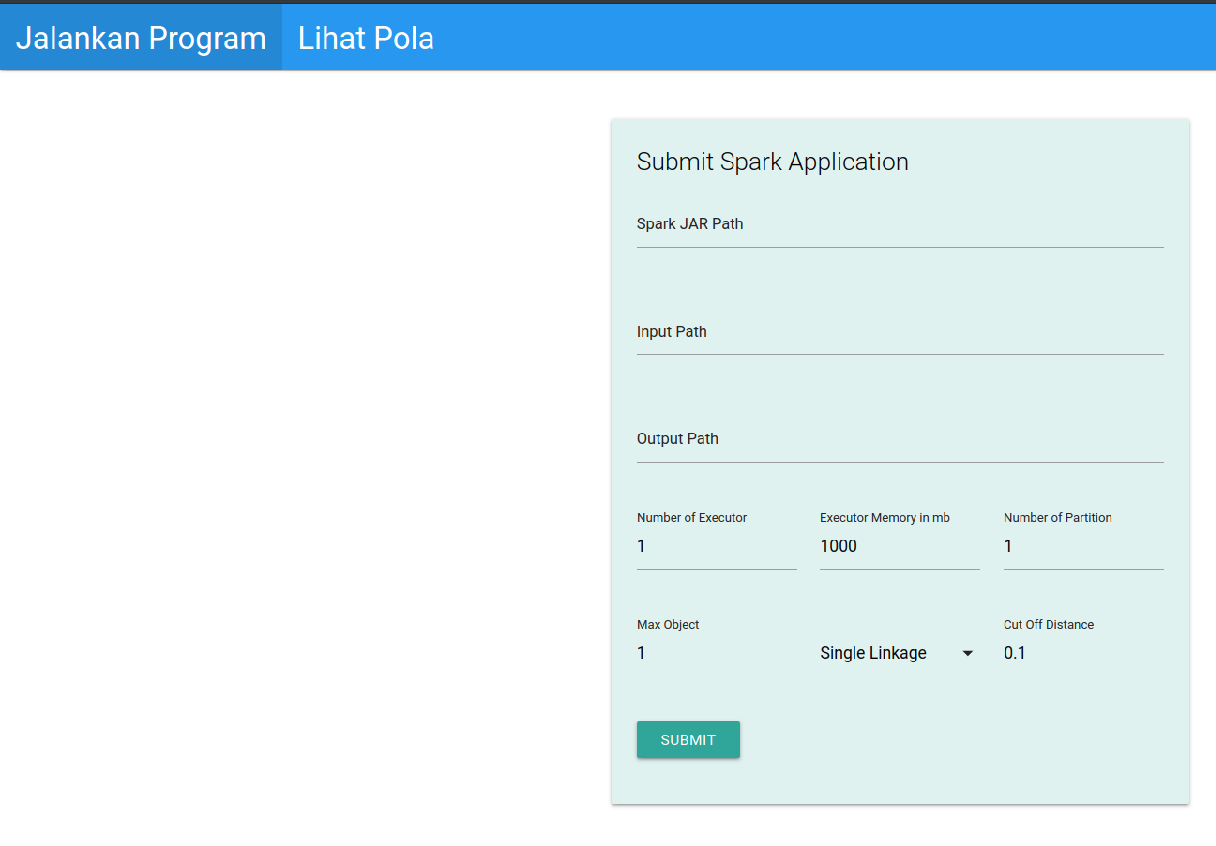
\includegraphics[scale=0.3]{menusubmit}  
    \caption[Tampilan menu \textit{Submit}]{Tampilan menu \textit{submit}} 
    \label{fig:menusubmit} 
\end{figure}

\item Implementasi antarmuka untuk menu \textit{Data} dapat dilihat pada Gambar ~\ref{fig:menudata}.

\begin{figure}[H]
    \centering  
    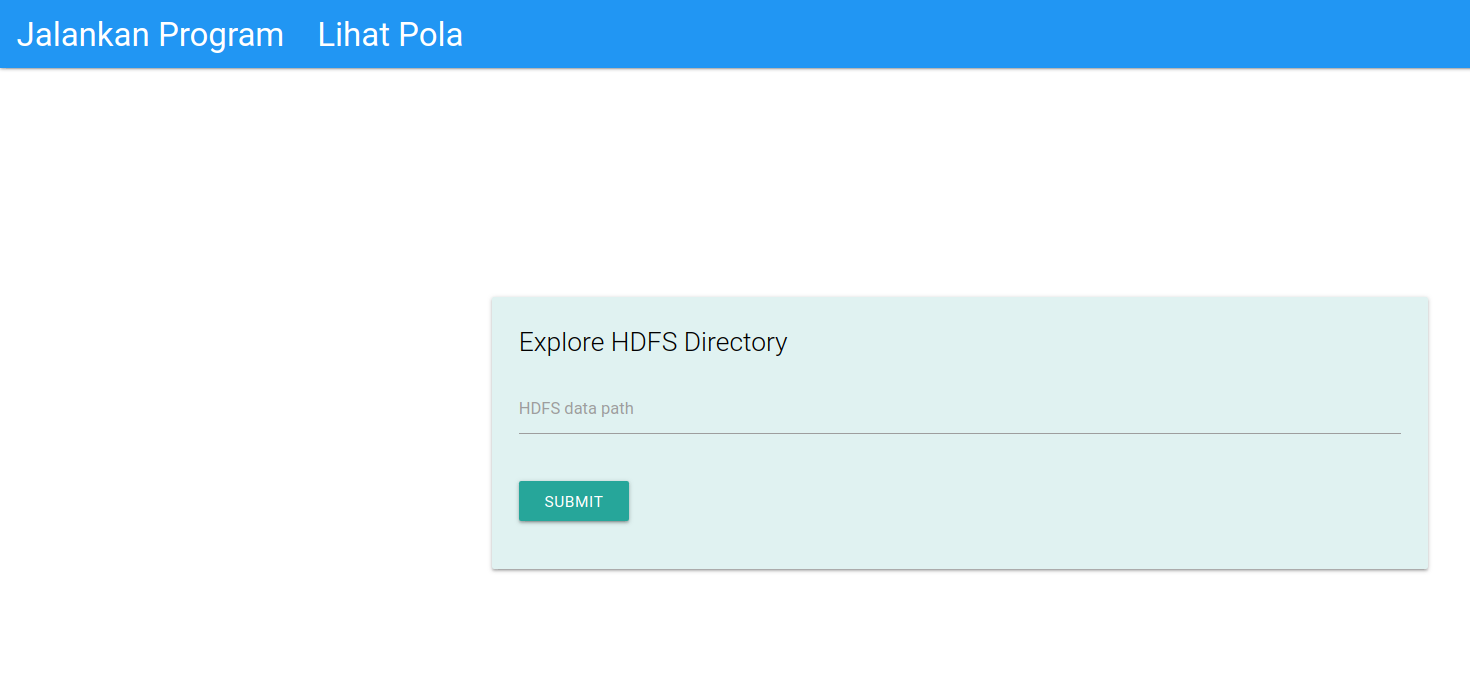
\includegraphics[scale=0.3]{menudata}  
    \caption[Tampilan menu \textit{Data}]{Tampilan menu \textit{Data}} 
    \label{fig:menudata} 
\end{figure}

\item Implementasi antarmuka sesudah melakukan \textit{submit} dapat dilihat pada Gambar ~\ref{fig:menuresult}.

\begin{figure}[H]
    \centering  
    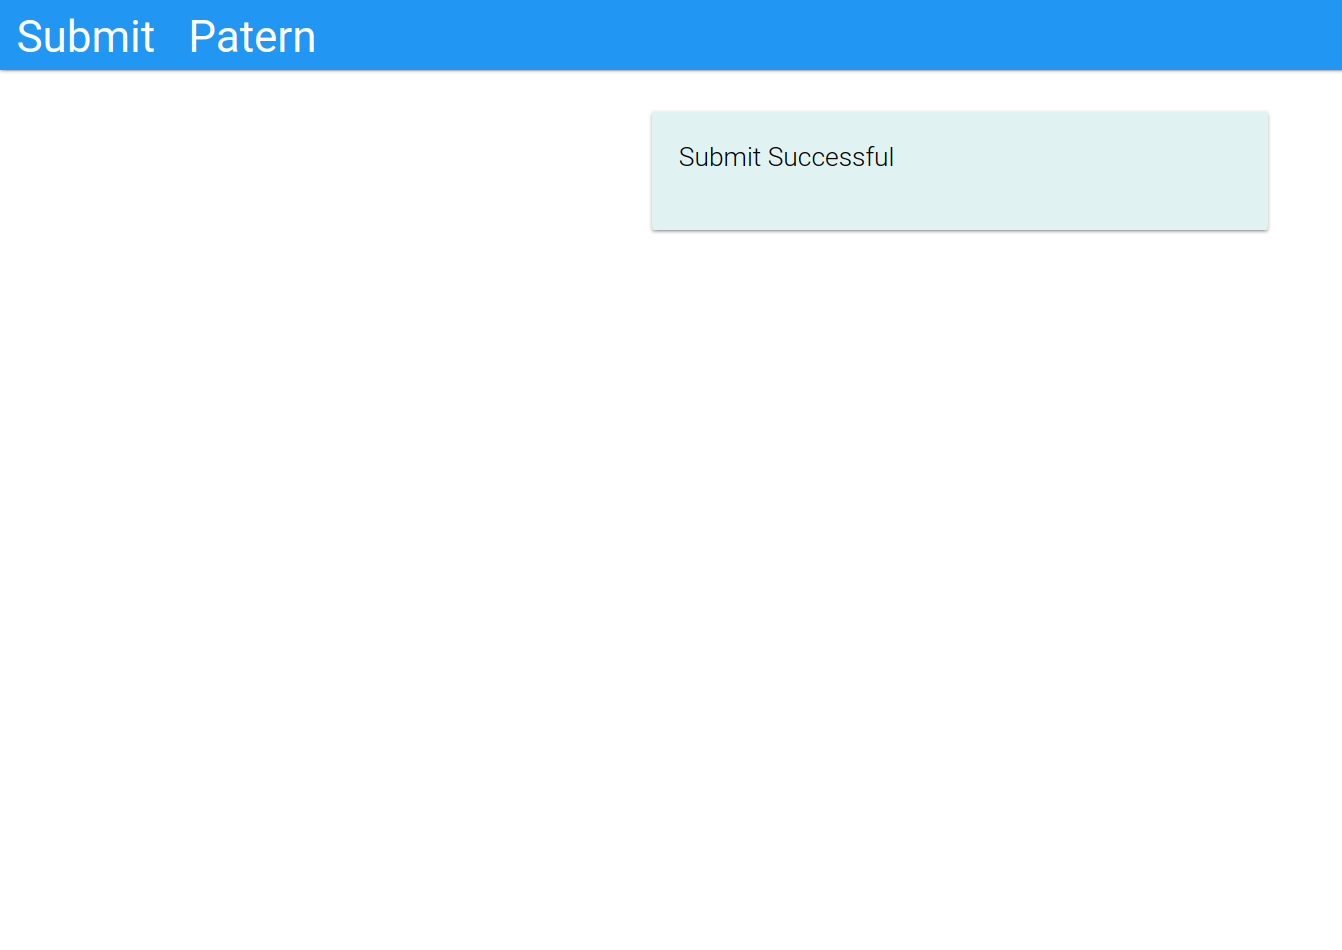
\includegraphics[scale=0.3]{menuresult}  
    \caption[Tampilan halaman sesudah \textit{submit}]{Tampilan halaman sesudah \textit{submit}} 
    \label{fig:menuresult} 
\end{figure}

\item Implementasi antarmuka  halaman \textit{list} dapat dilihat pada Gambar ~\ref{fig:menulist}.

\begin{figure}[H]
    \centering  
    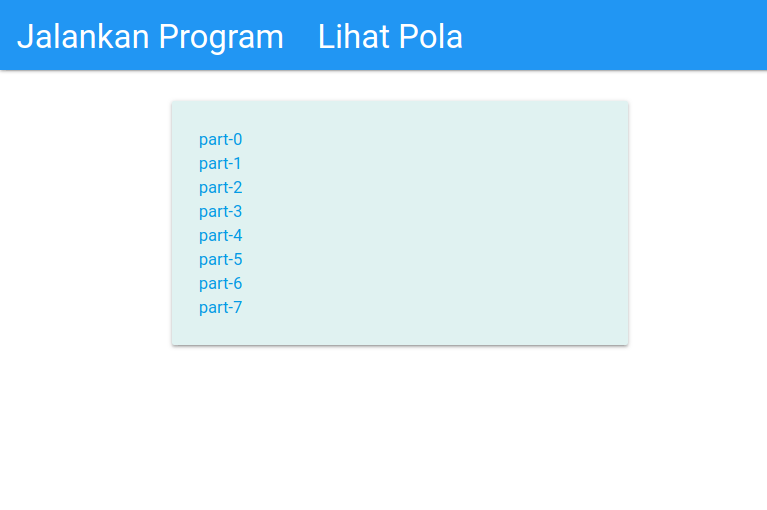
\includegraphics[scale=0.5]{menulist}  
    \caption[Tampilan halaman \textit{list}]{Tampilan halaman \textit{list}} 
    \label{fig:menulist} 
\end{figure}

\item Implementasi antarmuka  halaman \textit{data} dapat dilihat pada Gambar ~\ref{fig:menudata2}.

\begin{figure}[H]
    \centering  
    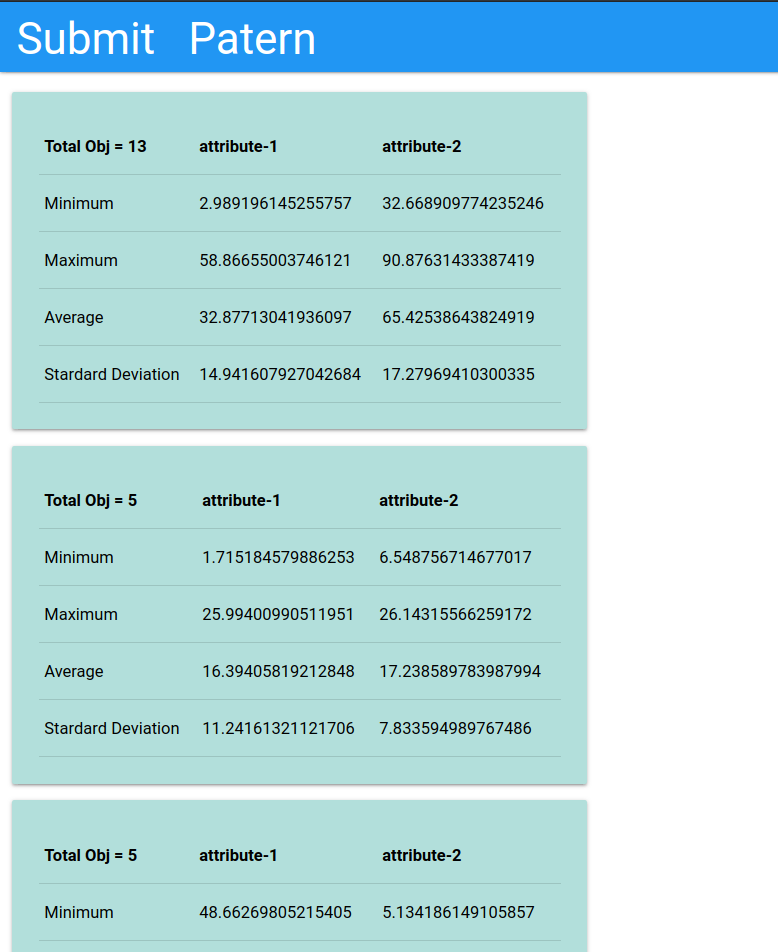
\includegraphics[scale=0.5]{menudata2}  
    \caption[Tampilan halaman data]{Tampilan halaman data} 
    \label{fig:menudata2} 
\end{figure}

\end{enumerate}

\section{Pengujian Fungsional Perangkat Lunak}

Perangkat lunak yang disusun oleh penulis telah diuji untuk membuktikan kebenaran dari perangkat lunak. Program akan dieksekusi dan kemudian diamati apakah hasil sesuai dengan yang diinginkan. Perangkat lunak akan diberikan data dengan ukuran yang kecil berserta \textit{parameter} yang sudah ditentukan. 

\begin{itemize}

\item Pada percobaan pertama, akan digunakan metode \textit{single linkage}, dengan jumlah partisi = 1, jumlah objek maksimum = 4, dan nilai \textit{cut-off distance} = 0.8. Berikut adalah data yang digunakan untuk pengujian:

\begin{verbatim}
4.0,5.0
3.0,7.0
4.0,3.0
10.0,7.0
10.0,10.0
\end{verbatim}

Hasil dari percobaan pertama adalah sebagai berikut:

\begin{verbatim}
3
3.0,3.0
4.0,7.0
3.6666666666666665,5.0
0.5773502691896258,2.0
1
10.0,7.0
10.0,7.0
10.0,7.0
0.0,0.0
1
10.0,10.0
10.0,10.0
10.0,10.0
0.0,0.0
\end{verbatim}

\item Pada percobaan kedua, akan digunakan metode \textit{complete linkage}, dengan jumlah partisi = 1, jumlah objek maksimum = 4, dan nilai \textit{cut-off distance} = 0.8. Berikut adalah data yang digunakan untuk pengujian:

\begin{verbatim}
4.0,5.0
3.0,7.0
4.0,3.0
10.0,7.0
10.0,10.0
\end{verbatim}

Hasil dari percobaan kedua adalah sebagai berikut:

\begin{verbatim}
3
3.0,3.0
4.0,7.0
3.6666666666666665,5.0
0.5773502691896258,2.0
1
10.0,7.0
10.0,7.0
10.0,7.0
0.0,0.0
1
10.0,10.0
10.0,10.0
10.0,10.0
0.0,0.0
\end{verbatim}

\item Pada percobaan ketiga, akan digunakan metode \textit{centroid linkage}, dengan jumlah partisi = 1, jumlah objek maksimum = 4, dan nilai \textit{cut-off distance} = 0.8. Berikut adalah data yang digunakan untuk pengujian:

\begin{verbatim}
4.0,5.0
3.0,7.0
4.0,3.0
10.0,7.0
10.0,10.0
\end{verbatim}

Hasil dari percobaan ketiga adalah sebagai berikut:

\begin{verbatim}
3
3.0,3.0
4.0,7.0
3.6666666666666665,5.0
0.5773502691896258,2.0
1
10.0,7.0
10.0,7.0
10.0,7.0
0.0,0.0
1
10.0,10.0
10.0,10.0
10.0,10.0
0.0,0.0
\end{verbatim}

 
\end{itemize}

Berdasarkan hasil ketiga percobaan yang didapat, maka dapat disimpulkan bahwa perangkat lunak sudah dapat melakukan proses reduksi data menggunakan algoritma \textit{Agglomerative Clustering} berdasarkan metode yang dipilih dengan benar. Pola yang dihasilkan oleh perangkat lunak sudah sesuai dengan apa yang diharapakan.

\section{Hasil Eksperimen Perangkat Lunak}

Pada bagian ini akan diuji performa perangkat lunak Spark dan Hadoop. Kedua perangkat lunak akan dibandingkan hasil eksekusi waktunya. Karena perangkat lunak hadoop tidak dapat menghitung standard deviasi, maka perangkat lunak Hadoop akan dibandingkan dengan perangkat lunak Spark yang tidak menghitung standard deviasi dan yang menghitung standard deviasi. Data yang digunakan pada percobaan merupakan data yang dihasilkan secara acak dengan ukuran yang berbeda-beda. Data-data tersebut memiliki dua atribut bilangan pecahan yang dipisahkan dengan tanda koma. Jumlah objek pada setiap ukuran data dapat dilihat pada Tabel ~\ref{tab:exdata}.\\

\begin{table}[H] 
	\centering 
	\caption{Tabel data yang digunakan pada eksperimen}
	\label{tab:exdata}
	\begin{tabular}{|p{2cm}|p{2cm}|p{4cm}|}
\hline
Ukuran Data & Jumlah Objek  & Jumlah Block\\
\hline
1 GB & 36000000 & 40 \\
\hline
2 GB & 64000000 & 70 \\
\hline
3 GB & 81000000 & 89 \\
\hline
5 GB & 144000000 & 157 \\
\hline
10 GB & 256000000 & 279 \\
\hline
15 GB & 400000000 & 435 \\
\hline
20 GB & 529000000 & 576 \\
\hline
	\end{tabular} 
\end{table}



Berikut adalah spesifikasi perangkat keras yang digunakan:

\begin{itemize}

\item \textit{Processor}: Intel core i5 8500 @3.00 GHz, 6 \textit{core}

\item RAM: 8GB

\item \textit{Harddisk}: 500GB

\item Sistem Operasi: Ubuntu 18.0.4

\end{itemize}






\section{Percobaan Dampak Partisi pada Performa Perangkat Lunak Spark dan Hadoop} 
%1111111111GBBBBBBBBBBBBBBBBB

Pada percobaan ini akan dilihat waktu ekseuksi Spark dan Hadoop berdasarkan jumlah partisi yang berbeda. Percobaan ini akan menggunakan 1 komputer sebagai komputer \textit{master} dan 10 komputer lainya sebagai \textit{worker} dengan setiap \textit{worker} munggunakan 1 core. Ukuran data yang digunakan adalah 1 GB. Metode yang dingunakan adalah metode \textit{single linkage}, dengan nilai \textit{cut-off distance} adalah 0,8 dan jumlah objek maksimum untuk setiap \textit{dendrogram} adalah 30. Tabel (~\ref{tab:spark1}) berikut adalah hasil dari eksperimen:

\begin{table}[H] 
	\centering 
	\caption{Percobaan Jumlah Partisi Hadoop dan Spark dengan Ukuran Data 10 GB}
	\label{tab:spark1}
	\begin{tabular}{|p{1.5cm}|p{1.5cm}|p{3cm}|p{3cm}|p{3cm}|p{2cm}|p{2cm}|p{2cm}|}
\hline
Ukuran Data (GB) & Jumlah Partisi &  Waktu Ekseuksi Spark Tanpa Standard Deviasi (Detik) & Waktu Eksekusi Spark (Detik) & Waktu Eksekusi Hadoop (Detik) & Hasil Reduksi Spark Tanpa Standard Deviasi (GB) & Hasil Reduksi Spark (GB)  & Hasil Reduksi Hadoop (GB)\\ 
\hline
1 GB & 10 & 319 & 304 & 214 & 0.54 & 0.67 & 0.57 \\
\hline
1 GB & 30 & 131 & 124 & 216 & 0.54 & 0.67 & 0.57 \\
\hline
1 GB & 50 & 101 & 89 & 230 & 0.54 & 0.67 & 0.57 \\
\hline
1 GB & 100 & 62 & 63 & 303 & 0.54 & 0.67 & 0.57 \\
\hline
1 GB & 150 & 56 & 56 & 313 & 0.54 & 0.67 & 0.57 \\
\hline

\hline

	\end{tabular} 
\end{table}




\def\scl{1}

\def\leg{} 
\def\std{none}
\def\ymin{}
\def\ymax{}

\begin{minipage}[c]{0.9\textwidth}
	\begin{figure}[H]
		\centering
		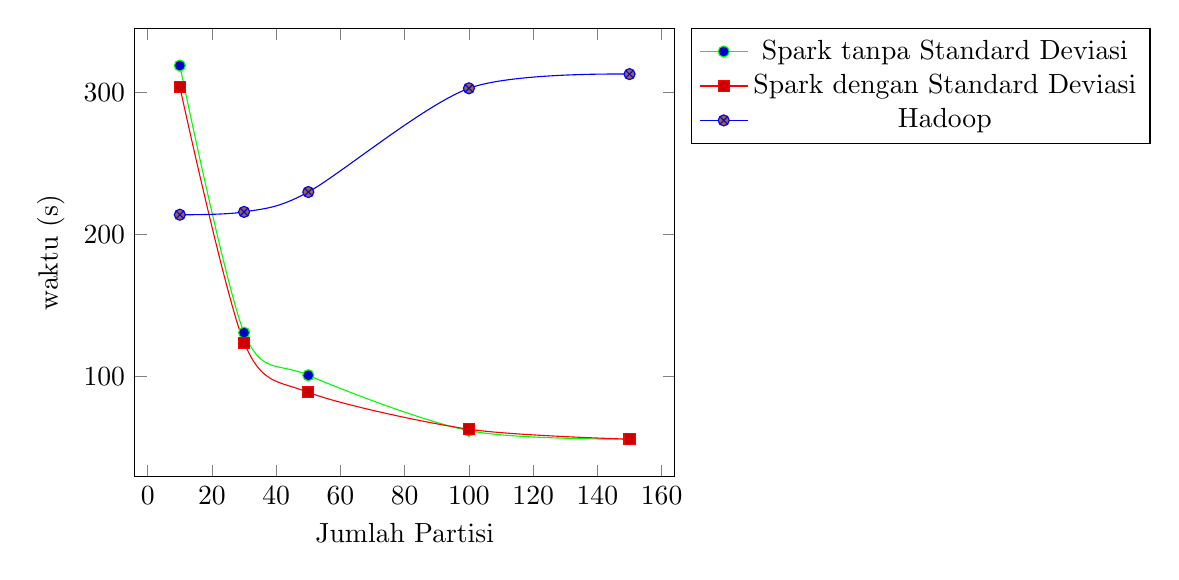
\begin{tikzpicture}[scale=\scl]
		\begin{axis}[\ymin,\ymax,xlabel= Jumlah Partisi,ylabel= waktu (s), xticklabel style={/pgf/number format/.cd, fixed,fixed zerofill, precision=0},legend pos = outer north east]
		
		\addlegendentry{Spark tanpa Standard Deviasi}
		\addplot+[smooth][color=green] coordinates {(10,319) (30,131) (50,101) (100,62) (150,56) };
		\addlegendentry{Spark dengan Standard Deviasi}
		\addplot+[smooth][color=red] coordinates {(10,304) (30,124) (50,89) (100,63) (150,56)};
		\addlegendentry{Hadoop}
		\addplot+[smooth][color=blue] coordinates {(10,214) (30,216) (50,230) (100,303) (150,313)};

		\leg
		\end{axis}
		\end{tikzpicture}
		\caption[Hasil percobaan partisi Spark dan Hadoop 1GB]{Hasil percobaan partisi Spark dan Hadoop 1GB}
		\label{fig:percobaan1}
	\end{figure}
\end{minipage}\\


%222222222222222222222GBBBBBBBBBBBBBBBBB

Pada percobaan ini akan dilihat waktu ekseuksi Spark dan Hadoop berdasarkan jumlah partisi yang berbeda. Percobaan ini akan menggunakan 1 komputer sebagai komputer master dan 10 komputer lainya sebagai worker dengan setiap worker munggunakan 1 core. Ukuran data yang digunakan adalah 2 GB. Metode yang dingunakan adalah metode \textit{single linkage}, dengan nilai \textit{cut-off distance} adalah 0,8 dan jumlah objek maksimum untuk setiap \textit{dendrogram} adalah 30. Tabel (~\ref{tab:spark2}) berikut adalah hasil dari eksperimen:

\begin{table}[H] 
	\centering 
	\caption{Percobaan Jumlah Partisi Hadoop dan Spark dengan Ukuran Data 2 GB}
	\label{tab:spark2}
	\begin{tabular}{|p{1.5cm}|p{1.5cm}|p{3cm}|p{3cm}|p{3cm}|p{2cm}|p{2cm}| p{2cm}|}
\hline
Ukuran Data (GB) & Jumlah Partisi &  Waktu Ekseuksi Spark Tanpa Standard Deviasi (Detik) & Waktu Eksekusi Spark (Detik) & Waktu Eksekusi Hadoop (Detik) & Hasil Reduksi Spark Tanpa Standard Deviasi (GB) & Hasil Reduksi Spark (GB)  & Hasil Reduksi Hadoop (GB)\\ 
\hline
2 GB & 10 & 929  & 958  & 365  & 0.96 & 1.2 & 1 \\
\hline
2 GB & 30 & 350  & 317  & 355  & 0.96 & 1.2 & 1 \\
\hline
2 GB & 50 & 205  & 217  & 428  & 0.96 & 1.2 & 1 \\
\hline
2 GB & 100 & 126  & 134  & 446  & 0.96 & 1.2 & 1 \\
\hline
2 GB & 150 & 110  & 109  & 489  & 0.96 & 1.2 & 1 \\
\hline
2 GB & 200 & 98  & 99  & 545  & 0.96 & 1.2 & 1 \\
\hline
2 GB & 250 & 83  & 86  & 589  & 0.96 & 1.2 & 1 \\
\hline

\hline

	\end{tabular} 
\end{table}



\def\scl{1}

\def\leg{} 
\def\std{none}
\def\ymin{}
\def\ymax{}

\begin{minipage}[c]{0.9\textwidth}
	\begin{figure}[H]
		\centering
		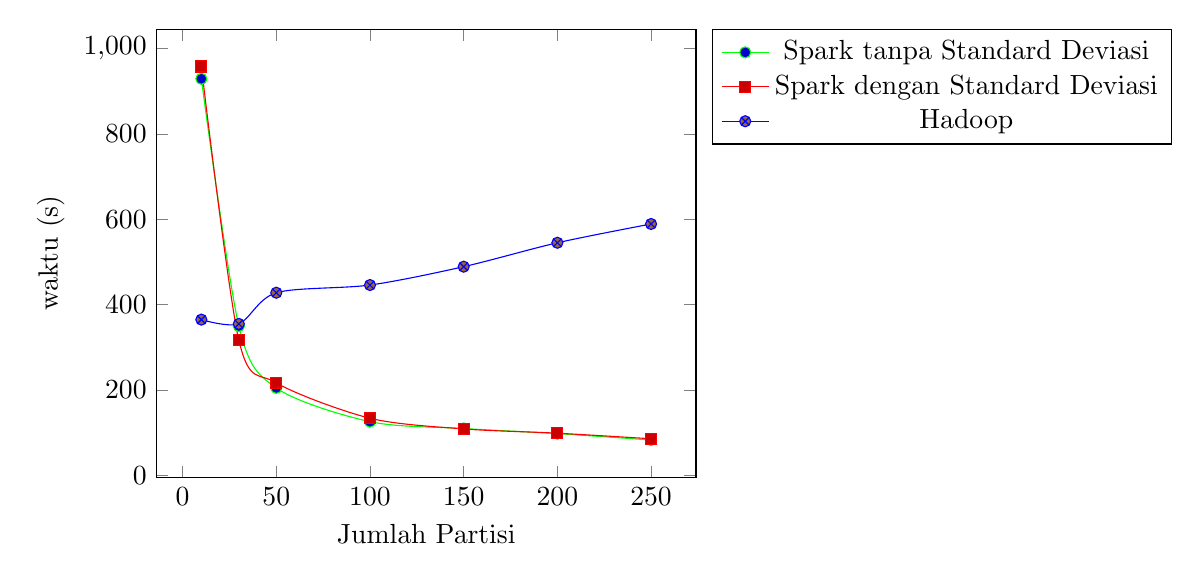
\begin{tikzpicture}[scale=\scl]
		\begin{axis}[\ymin,\ymax,xlabel= Jumlah Partisi,ylabel= waktu (s), xticklabel style={/pgf/number format/.cd, fixed,fixed zerofill, precision=0},legend pos = outer north east]
		
		\addlegendentry{Spark tanpa Standard Deviasi}
		\addplot+[smooth][color=green] coordinates {(10,929) (30,350) (50,205) (100,126) (150,110) (200,98) (250,83)};
		\addlegendentry{Spark dengan Standard Deviasi}
		\addplot+[smooth][color=red] coordinates {
		(10,958) (30,317) (50,217) (100,134) (150,109) (200,99) (250,86)};
		\addlegendentry{Hadoop}
		\addplot+[smooth][color=blue] coordinates {(10,365) (30,355) (50,428) (100,446) (150,489) (200,545) (250,589)};

		

		\leg
		\end{axis}
		\end{tikzpicture}
		\caption[Hasil percobaan partisi Spark dan Hadoop 2GB]{Hasil percobaan partisi Spark dan Hadoop 2GB}
		\label{fig:percobaan2}
	\end{figure}
\end{minipage}\\




%333333333333333333GBBBBBBBBBBBBBBBBB


Pada percobaan ini akan dilihat waktu ekseuksi Spark dan Hadoop berdasarkan jumlah partisi yang berbeda. Percobaan ini akan menggunakan 1 komputer sebagai komputer master dan 10 komputer lainya sebagai worker dengan setiap worker munggunakan 1 core. Ukuran data yang digunakan adalah 3 GB. Metode yang dingunakan adalah metode \textit{single linkage}, dengan nilai \textit{cut-off distance} adalah 0,8 dan jumlah objek maksimum untuk setiap \textit{dendrogram} adalah 30. Tabel (~\ref{tab:spark3}) berikut adalah hasil dari eksperimen:

\begin{table}[H] 
	\centering 
	\caption{Percobaan Jumlah Partisi Hadoop dan Spark dengan Ukuran Data 3 GB}
	\label{tab:spark3}
	\begin{tabular}{|p{1cm}|p{1cm}|p{2cm}|p{2cm}|p{2cm}|p{2cm}|p{2cm}|p{2cm}|}
\hline
Ukuran Data (GB) & Jumlah Partisi &  Waktu Ekseuksi Spark Tanpa Standard Deviasi (Detik) & Waktu Eksekusi Spark (Detik) & Waktu Eksekusi Hadoop (Detik) & Hasil Reduksi Spark Tanpa Standard Deviasi (GB) & Hasil Reduksi Spark (GB)  & Hasil Reduksi Hadoop (GB)\\ 
\hline
3 & 10 & 1446 & 1376 & 455 & 1.2 & 1.5 & 1.2 \\
\hline
3 & 30 & 516 & 491 & 445 & 1.2 & 1.5 & 1.2 \\
\hline
3 & 50 & 315 & 298 & 501 & 1.2 & 1.5 & 1.2 \\
\hline
3 & 100 & 188 & 183 & 532 & 1.2 & 1.5 & 1.2 \\
\hline
3 & 150 & 144 & 146 & 639 & 1.2 & 1.5 & 1.2 \\
\hline
3 & 200 & 135 & 144 & 720 & 1.2 & 1.5 & 1.2 \\
\hline
3 & 250 & 211 & 191 & 761 & 1.2 & 1.5 & 1.2 \\
\hline
3 & 300 & 182 & 176 & 822 & 1.2 & 1.5 & 1.2 \\
\hline
3 & 350 & 163 & 169 & 903 & 1.2 & 1.5 & 1.2 \\
\hline
3 & 400 & 137 & 158 & 1012 & 1.2 & 1.5 & 1.2 \\
\hline


\hline

	\end{tabular} 
\end{table}



\def\scl{1}

\def\leg{} 
\def\std{none}
\def\ymin{}
\def\ymax{}

\begin{minipage}[c]{0.9\textwidth}
	\begin{figure}[H]
		\centering
		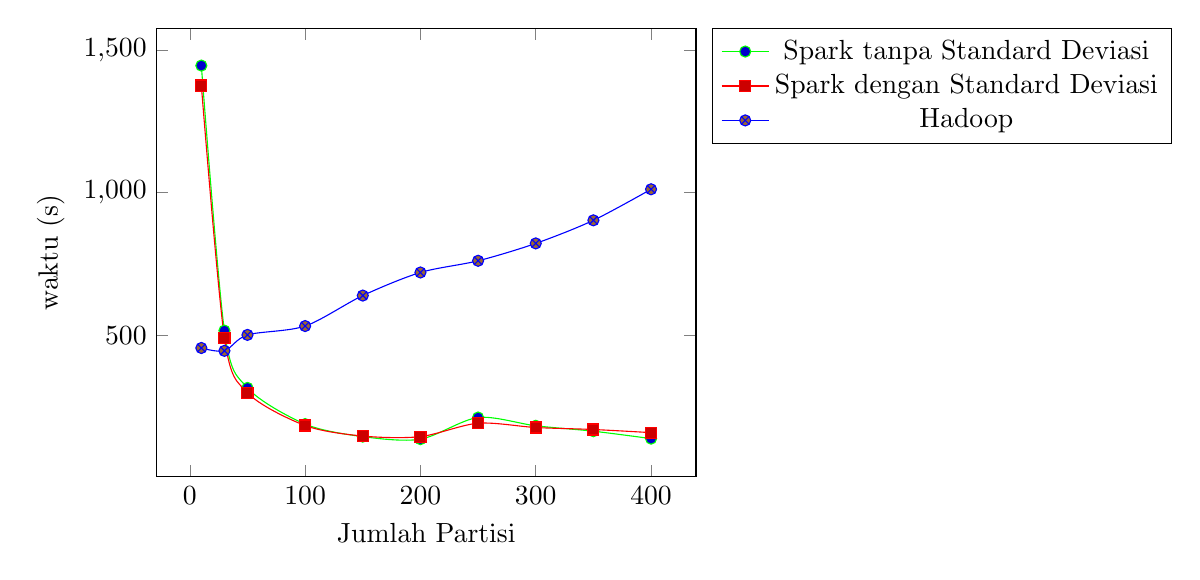
\begin{tikzpicture}[scale=\scl]
		\begin{axis}[\ymin,\ymax,xlabel= Jumlah Partisi,ylabel= waktu (s), xticklabel style={/pgf/number format/.cd, fixed,fixed zerofill, precision=0},legend pos = outer north east]
		
		\addlegendentry{Spark tanpa Standard Deviasi}
		\addplot+[smooth][color=green] coordinates {(10,1446) (30,516) (50,315) (100,188) (150,144) (200,135) (250,211) (300,182) (350,163) (400,137)};
		\addlegendentry{Spark dengan Standard Deviasi}
		\addplot+[smooth][color=red] coordinates {
		(10,1376) (30,491) (50,298) (100,183) (150,146) (200,144) (250,191) (300,176) (350,169) (400,158)};
		\addlegendentry{Hadoop}
		\addplot+[smooth][color=blue] coordinates {(10,455) (30,445) (50,501) (100,532) (150,639) (200,720) (250,761) (300,822) (350,903) (400,1012)};

		

		\leg
		\end{axis}
		\end{tikzpicture}
		\caption[Hasil percobaan partisi Spark dan Hadoop 3GB]{Hasil percobaan partisi Spark dan Hadoop 3GB}
		\label{fig:percobaan3}
	\end{figure}
\end{minipage}\\



%555555555555GBBBBBBBBBBBBBBBBB


Pada percobaan ini akan dilihat waktu ekseuksi Spark dan Hadoop berdasarkan jumlah partisi yang berbeda. Percobaan ini akan menggunakan 1 komputer sebagai komputer master dan 10 komputer lainya sebagai worker dengan setiap worker munggunakan 1 core. Ukuran data yang digunakan adalah 5 GB. Metode yang dingunakan adalah metode \textit{single linkage}, dengan nilai \textit{cut-off distance} adalah 0,8 dan jumlah objek maksimum untuk setiap \textit{dendrogram} adalah 30. Tabel (~\ref{tab:spark5}) berikut adalah hasil dari eksperimen:

\begin{table}[H] 
	\centering 
	\caption{Percobaan Jumlah Partisi Hadoop dan Spark dengan Ukuran Data 5 GB}
	\label{tab:spark5}
	\begin{tabular}{|p{1cm}|p{1cm}|p{2cm}|p{2cm}|p{2cm}|p{2cm}|p{2cm}|p{2cm}|}
\hline
Ukuran Data (GB) & Jumlah Partisi &  Waktu Ekseuksi Spark Tanpa Standard Deviasi (Detik) & Waktu Eksekusi Spark (Detik) & Waktu Eksekusi Hadoop (Detik) & Hasil Reduksi Spark Tanpa Standard Deviasi (GB) & Hasil Reduksi Spark (GB)  & Hasil Reduksi Hadoop (GB)\\ 
\hline
5  & 10 & 4490 & 4457 & 817 & 2.1 & 2.6 & 2.2\\
\hline
5  & 30 & 1637 & 2002 & 759 & 2.1 & 2.6 & 2.2\\
\hline
5  & 50 & 995 & 891 & 906 & 2.1 & 2.6 & 2.2 \
\hline
5  & 100 & 524 & 590 & 952 & 2.1 & 2.6 & 2.2 \
\hline
5  & 150 & 343 & 431 & 1121 & 2.1 & 2.6 & 2.2\\
\hline
5  & 200 & 315 & 288 & 1173 & 2.1 & 2.6 & 2.2\\
\hline
5  & 300 & 519 & 526 & 1485 & 2.1 & 2.6 & 2.2\\
\hline
5  & 400 & 422 & 399 & 2261 & 2.1 & 2.6 & 2.2 \\
\hline
5  & 500 & 359 & 370 & 1994 & 2.1 & 2.6 & 2.2\\
\hline
5  & 600 & 319 & 326 & 2282 & 2.1 & 2.6 & 2.2\\
\hline
5  & 700 & 259 & 306 & 2569 & 2.1 & 2.6 & 2.2\\
\hline
5  & 800 & 255 & 256 & 4463 & 2.1 & 2.6 & 2.2\\
\hline


\hline

	\end{tabular} 
\end{table}




\def\scl{1}

\def\leg{} 
\def\std{none}
\def\ymin{}
\def\ymax{}

\begin{minipage}[c]{0.9\textwidth}
	\begin{figure}[H]
		\centering
		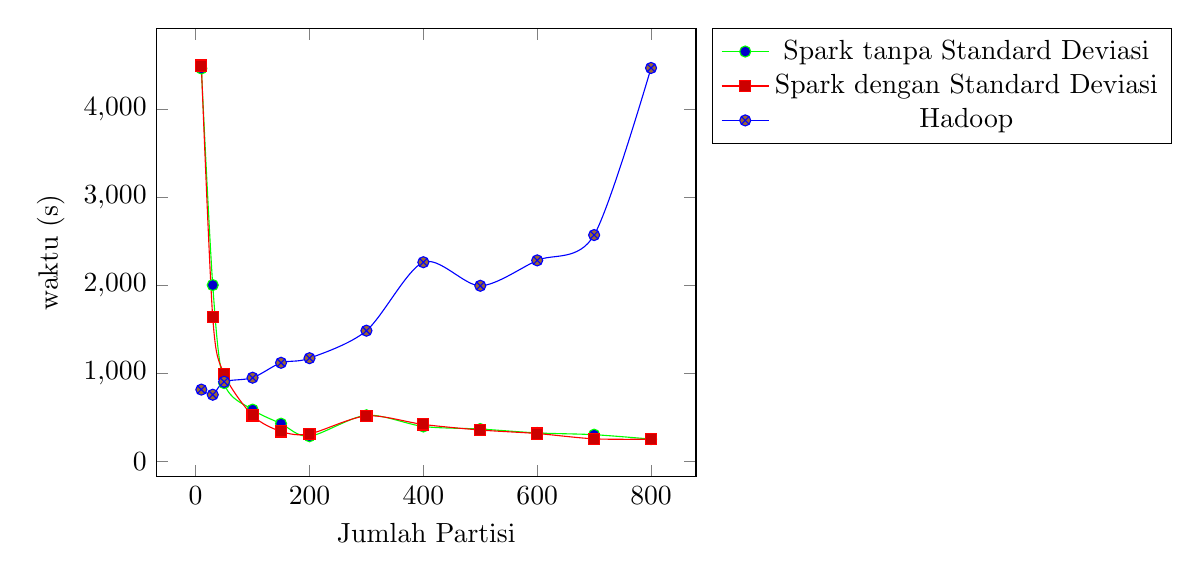
\begin{tikzpicture}[scale=\scl]
		\begin{axis}[\ymin,\ymax,xlabel= Jumlah Partisi,ylabel= waktu (s), xticklabel style={/pgf/number format/.cd, fixed,fixed zerofill, precision=0},legend pos = outer north east]
		
		\addlegendentry{Spark tanpa Standard Deviasi}
		\addplot+[smooth][color=green] coordinates {(10,4457) (30,2002) (50,891) (100,590) (150,431) (200,288) (300,526) (400,399) (500,370) (600,326) (700,306) (800,256)};
		\addlegendentry{Spark dengan Standard Deviasi}
		\addplot+[smooth][color=red] coordinates {(10,4490) (30,1637) (50,995) (100,524) (150,343) (200,315) (300,519) (400,422) (500,359) (600,319) (700,259) (800,255)};
		\addlegendentry{Hadoop}
		\addplot+[smooth][color=blue] coordinates {(10,817) (30,759) (50,906) (100,952) (150,1121) (200,1173) (300,1485) (400,2261) (500,1994) (600,2282) (700,2569) (800,4463)};

		

		\leg
		\end{axis}
		\end{tikzpicture}
		\caption[Hasil percobaan partisi Spark dan Hadoop 5GB]{Hasil percobaan partisi Spark dan Hadoop 5GB}
		\label{fig:percobaan2}
	\end{figure}
\end{minipage}\\





%100000000000000000GBBBBBBBBBBBBBBBBB



Pada percobaan ini akan dilihat waktu ekseuksi Spark dan Hadoop berdasarkan jumlah partisi yang berbeda. Percobaan ini akan menggunakan 1 komputer sebagai komputer master dan 10 komputer lainya sebagai worker dengan setiap worker munggunakan 1 core. Ukuran data yang digunakan adalah 10 GB. Metode yang dingunakan adalah metode \textit{single linkage}, dengan nilai \textit{cut-off distance} adalah 0,8 dan jumlah objek maksimum untuk setiap \textit{dendrogram} adalah 30. Tabel~\ref{tab:spark6} dan Tabel~\ref{tab:spark7} berikut adalah hasil dari eksperimen:

\begin{table}[H] 
	\centering 
	\caption{Percobaan Jumlah Partisi Hadoop dengan Ukuran Data 10 GB}
	\label{tab:spark6}
	\begin{tabular}{|p{1cm}|p{1cm}|p{3cm}|p{3cm}|p{3cm}|p{3cm}|}
\hline
Ukuran Data (GB) & Jumlah Partisi &  Waktu Ekseuksi Spark Tanpa Standard Deviasi (Detik) & Waktu Eksekusi Spark (Detik) & Hasil Reduksi Spark Tanpa Standard Deviasi (GB) & Hasil Reduksi Spark (GB)  \\ 
\hline
10 & 50 & 7254 & 7236 & 3.7 & 4.6 \\
\hline
10 & 100 & 237 & 2805 &  3.7 & 4.6 \\
\hline
10 & 200 & 1736 & 1718 & 3.7 & 4.6 \\
\hline
10 & 300 & 1477 & 1494 & 3.7 & 4.6 \\
\hline
10 & 400 & 1160 & 1207 & 3.7 & 4.6 \\
\hline
10 & 500 & 923 & 984 &  3.7 & 4.6 \\
\hline
10 & 600 & 774 & 780 & 3.7 & 4.6 \\
\hline
10 & 700 & 645 & 652 & 3.7 & 4.6 \\
\hline
10 & 900 & 563 & 568 & 3.7 & 4.6 \\
\hline
10 & 1100 & 522 & 524 & 3.7 & 4.6 \\
\hline
10 & 1300 & 359 & 504 & 3.7 & 4.6 \\
\hline
10 & 1500 & 255 & 256 & 3.7 & 4.6 \\
\hline


\hline

	\end{tabular} 
\end{table}



\begin{table}[H] 
	\centering 
	\caption{Percobaan Jumlah Partisi Hadoop dengan Ukuran Data 10 GB}
	\label{tab:spark7}
	\begin{tabular}{|p{3cm}|p{3cm}|p{4cm}|p{4cm}|}
\hline
Ukuran Data (GB) & Jumlah Partisi &  Waktu Eksekusi Hadoop (Detik) & Hasil Reduksi Hadoop (GB)\\
\hline
10 & 10  & 3.9 \\
\hline
10 & 30  & 3.9 \\
\hline
10 & 50  & 3.9 \\
\hline
10 & 100  & 3.9 \\
\hline
10 & 200  & 3.9 \\
\hline
10 & 300  & 3.9 \\
\hline
10 & 400  & 3.9 \\
\hline
10 & 500  & 3.9 \\
\hline
10 & 700  & 3.9 \\
\hline
10 & 900  & 3.9 \\
\hline
10 & 1100  & 3.9 \\
\hline
10 & 1300  & 3.9 \\
\hline
10 & 1500  & 3.9 \\
\hline


\hline

	\end{tabular} 
\end{table}



\def\scl{1}

\def\leg{} 
\def\std{none}
\def\ymin{}
\def\ymax{}

\begin{minipage}[c]{0.9\textwidth}
	\begin{figure}[H]
		\centering
		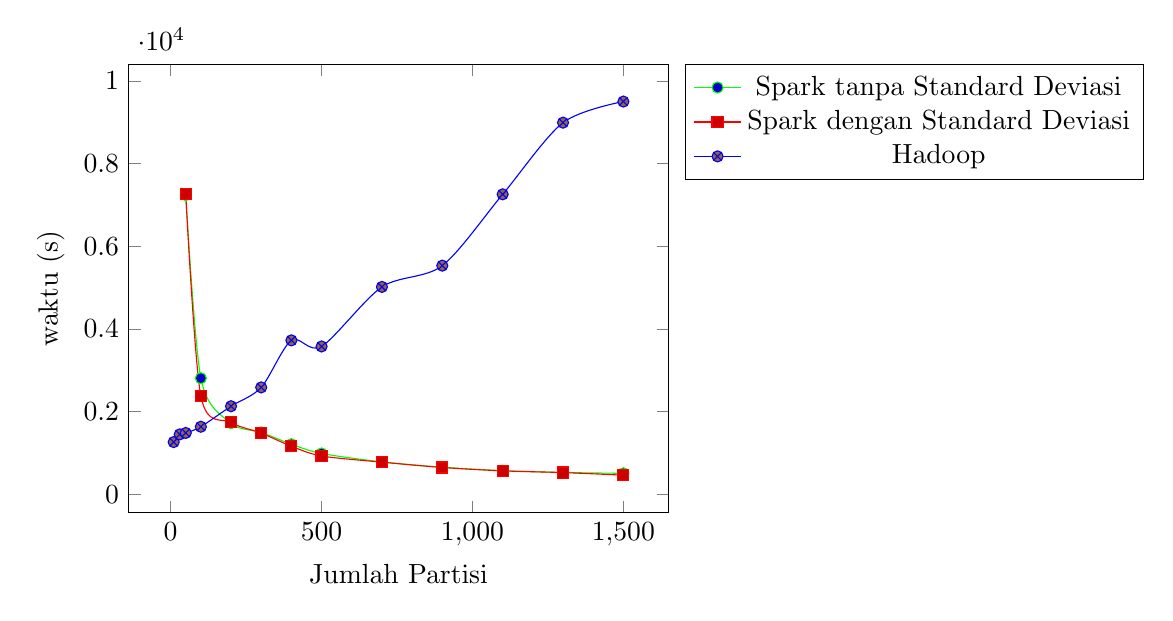
\begin{tikzpicture}[scale=\scl]
		\begin{axis}[\ymin,\ymax,xlabel= Jumlah Partisi,ylabel= waktu (s), xticklabel style={/pgf/number format/.cd, fixed,fixed zerofill, precision=0},legend pos = outer north east]
		
		\addlegendentry{Spark tanpa Standard Deviasi}
		\addplot+[smooth][color=green] coordinates {(50,7236) (100,2805) (200,1718) (300,1494) (400,1207) (500,984) (700,780) (900,652) (1100,568) (1300,524) (1500,504)};
		\addlegendentry{Spark dengan Standard Deviasi}
		\addplot+[smooth][color=red] coordinates {(50,7254) (100,2373) (200,1736) (300,1477) (400,1160) (500,923) (700,774) (900,645) (1100,563) (1300,522) (1500,459)};
		\addlegendentry{Hadoop}
		\addplot+[smooth][color=blue] coordinates {(10,1260) (30,1446) (50,1481) (100,1631) (200,2127) (300,2583) (400,3721) (500,3573) (700,5014) (900,5529) (1100,7254) (1300,8989) (1500,9499)};

		

		\leg
		\end{axis}
		\end{tikzpicture}
		\caption[Hasil percobaan partisi Spark dan Hadoop 10GB]{Hasil percobaan partisi Spark dan Hadoop 10GB}
		\label{fig:percobaan2}
	\end{figure}
\end{minipage}\\






%1111111111555555555555GBBBBBBBBBBBBBBBBB


Pada percobaan ini akan dilihat waktu ekseuksi Spark dan Hadoop berdasarkan jumlah partisi yang berbeda. Percobaan ini akan menggunakan 1 komputer sebagai komputer master dan 10 komputer lainya sebagai worker dengan setiap worker munggunakan 1 core. Ukuran data yang digunakan adalah 15 GB. Metode yang dingunakan adalah metode \textit{single linkage}, dengan nilai \textit{cut-off distance} adalah 0,8 dan jumlah objek maksimum untuk setiap \textit{dendrogram} adalah 30. Tabel (~\ref{tab:spark7} dan Tabel (~\ref{tab:spark8}) berikut adalah hasil dari eksperimen:

\begin{table}[H] 
	\centering 
	\caption{Percobaan Jumlah Partisi Hadoop dengan Ukuran Data 15}
	\label{tab:spark7}
	\begin{tabular}{|p{1cm}|p{1cm}|p{3cm}|p{3cm}|p{3cm}|p{3cm}|}
\hline
Ukuran Data ) & Jumlah Partisi &  Waktu Ekseuksi Spark Tanpa Standard Deviasi (GB) & Waktu Eksekusi Spark (detik) & Hasil Reduksi Spark Tanpa Standard Deviasi ) & Hasil Reduksi Spark )  \\ 
\hline
15 & 100 & 9034  & 9294  &  5.8 & 7.3 \\
\hline
15 & 200 & 5239  & 4847  & 5.8 & 7.3 \\
\hline
15 & 300 & 3263  & 3761  & 5.8 & 7.3 \\
\hline
15 & 500 & 2175  & 2024  &  5.8 & 7.3 \\
\hline
15 & 700 & 1645  & 1696  & 5.8 & 7.3 \\
\hline
15 & 900 & 1276  & 1372  & 5.8 & 7.3 \\
\hline
15 & 1200 & 1136  & 1114  & 5.8 & 7.3 \\
\hline
15 & 1500 & 970  & 918  & 5.8 & 7.3 \\
\hline
15 & 1800 & 834  & 863  & 5.8 & 7.3 \\
\hline
15 & 2100 & 773  & 783  & 5.8 & 7.3 \\
\hline
15 & 2400 & 739  & 738  & 5.8 & 7.3 \\
\hline

\hline

	\end{tabular} 
\end{table}



\begin{table}[H] 
	\centering 
	\caption{Percobaan Jumlah Partisi Hadoop dengan Ukuran Data 15 GB}
	\label{tab:spark8}
	\begin{tabular}{|p{3cm}|p{3cm}|p{4cm}|p{4cm}|}
\hline
Ukuran Data (GB) & Jumlah Partisi &  Waktu Eksekusi Hadoop (detik) & Hasil Reduksi Hadoop (GB)\\
\hline
15 & 10 & 2133  & 3.9 \\
\hline
15 & 30 & 2177  & 3.9 \\
\hline
15 & 50 & 2234  & 3.9 \\
\hline
15 & 100 & 2474  & 3.9 \\
\hline
15 & 200 & 3306  & 3.9 \\
\hline
15 & 300 & 4655  & 3.9 \\
\hline
15 & 400 & 4775  & 3.9 \\
\hline
15 & 500 & 6644  & 3.9 \\
\hline
15 & 700 & 8203  & 3.9 \\
\hline
15 & 900 & 8482  & 3.9 \\
\hline


\hline

	\end{tabular} 
\end{table}


\def\scl{1}

\def\leg{} 
\def\std{none}
\def\ymin{}
\def\ymax{}

\begin{minipage}[c]{0.9\textwidth}
	\begin{figure}[H]
		\centering
		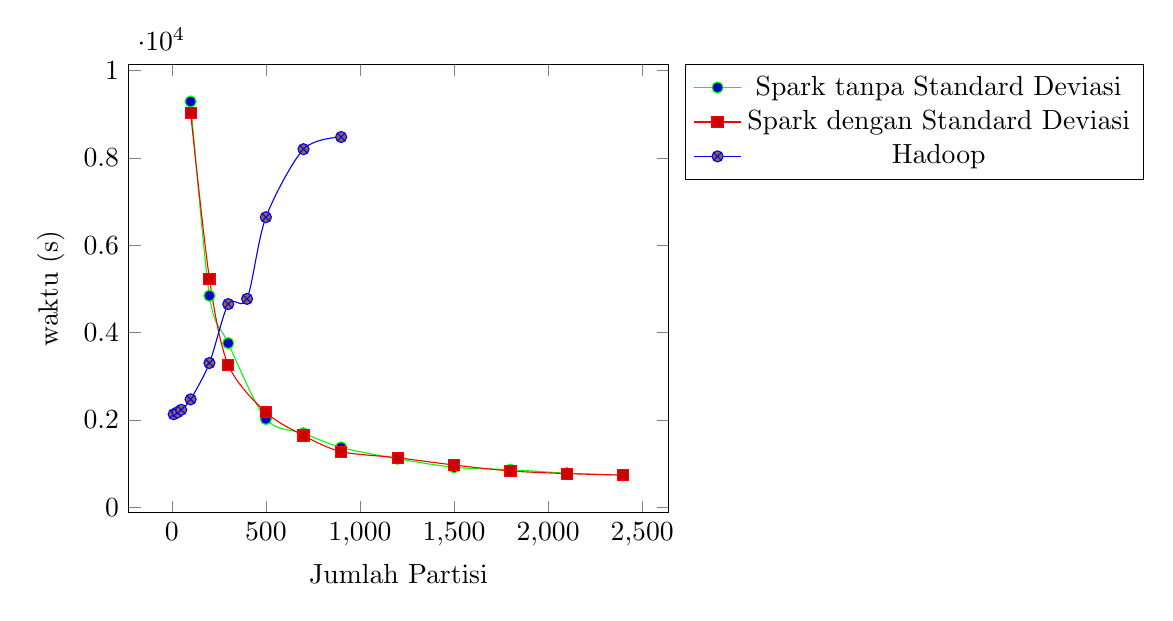
\begin{tikzpicture}[scale=\scl]
		\begin{axis}[\ymin,\ymax,xlabel= Jumlah Partisi,ylabel= waktu (s), xticklabel style={/pgf/number format/.cd, fixed,fixed zerofill, precision=0},legend pos = outer north east]
		
		\addlegendentry{Spark tanpa Standard Deviasi}
		\addplot+[smooth][color=green] coordinates { (100,9294) (200,4847) (300,3761) (500,2024) (700,1696) (900,1372) (1200,1114) (1500,918) (1800,863) (2100,783) (2400,738)};
		\addlegendentry{Spark dengan Standard Deviasi}
		\addplot+[smooth][color=red] coordinates {(100,9034) (200,5239) (300,3263) (500,2175) (700,1645) (900,1276) (1200,1136) (1500,970) (1800,834) (2100,773) (2400,739)};
		\addlegendentry{Hadoop}
		\addplot+[smooth][color=blue] coordinates {(10,2133) (30,2177) (50,2234) (100,2474) (200,3306) (300,4655) (400,4775) (500,6644) (700,8203) (900,8482)};

		

		\leg
		\end{axis}
		\end{tikzpicture}
		\caption[Hasil percobaan partisi Spark dan Hadoop 15GB]{Hasil percobaan partisi Spark dan Hadoop 15GB}
		\label{fig:percobaan2}
	\end{figure}
\end{minipage}\\




%2222222222222200000000000000000GBBBBBBBBBBBBBBBBB


Pada percobaan ini akan dilihat waktu ekseuksi Spark dan Hadoop berdasarkan jumlah partisi yang berbeda. Percobaan ini akan menggunakan 1 komputer sebagai komputer master dan 10 komputer lainya sebagai worker dengan setiap worker munggunakan 1 core. Ukuran data yang digunakan adalah 20 GB. Metode yang dingunakan adalah metode \textit{single linkage}, dengan nilai \textit{cut-off distance} adalah 0,8 dan jumlah objek maksimum untuk setiap \textit{dendrogram} adalah 30. Tabel (~\ref{tab:spark9} dan Tabel (~\ref{tab:spark10}) berikut adalah hasil dari eksperimen:

\begin{table}[H] 
	\centering 
	\caption{Percobaan Jumlah Partisi Hadoop dengan Ukuran Data 20}
	\label{tab:spark9}
	\begin{tabular}{|p{1cm}|p{1cm}|p{3cm}|p{3cm}|p{3cm}|p{3cm}|}
\hline
Ukuran Data (GB) & Jumlah Partisi &  Waktu Ekseuksi Spark Tanpa Standard Deviasi (detik) & Waktu Eksekusi Spark (detik) & Hasil Reduksi Spark Tanpa Standard Deviasi (GB) & Hasil Reduksi Spark (GB)  \\ 
\hline
20 & 200 & 8866  & 8386  & 7.7 & 9.6 \\
\hline
20 & 400 & 4553  & 4342  & 7.7 & 9.6 \\
\hline
20 & 600 & 3021  & 2841  &  7.7 & 9.6 \\
\hline
20 & 1000 & 2084  & 2065  & 7.7 & 9.6 \\
\hline
20 & 1400 & 1471  & 1598  & 7.7 & 9.6 \\
\hline
20 & 1800 & 1298  & 1372  & 7.7 & 9.6 \\
\hline
20 & 2200 & 1165  & 1228  & 7.7 & 9.6 \\
\hline
20 & 2600 & 1081  & 1133  & 7.7 & 9.6 \\
\hline
20 & 3000 & 1031  & 1010  & 7.7 & 9.6 \\
\hline

\hline

	\end{tabular} 
\end{table}



\begin{table}[H] 
	\centering 
	\caption{Percobaan Jumlah Partisi Hadoop dengan Ukuran Data 20 GB}
	\label{tab:spark10}
	\begin{tabular}{|p{3cm}|p{3cm}|p{4cm}|p{4cm}|}
\hline
Ukuran Data (GB) & Jumlah Partisi &  Waktu Eksekusi Hadoop (detik) & Hasil Reduksi Hadoop (GB)\\
\hline
20 & 10 & 2763  & 8.1 \\
\hline
20 & 30 & 2811  & 8.1 \\
\hline
20 & 50 & 3007  & 8.1  \\
\hline
20 & 100 & 3261  & 8.1 \\
\hline
20 & 200 & 4360  & 8.1 \\
\hline
20 & 400 & 6249  & 8.1 \\
\hline
20 & 700 & 10476  & 8.1 \\
\hline
20 & 1000 & 13839  & 8.1 \\
\hline


\hline

	\end{tabular} 
\end{table}



\def\scl{1}

\def\leg{} 
\def\std{none}
\def\ymin{}
\def\ymax{}

\begin{minipage}[c]{0.9\textwidth}
	\begin{figure}[H]
		\centering
		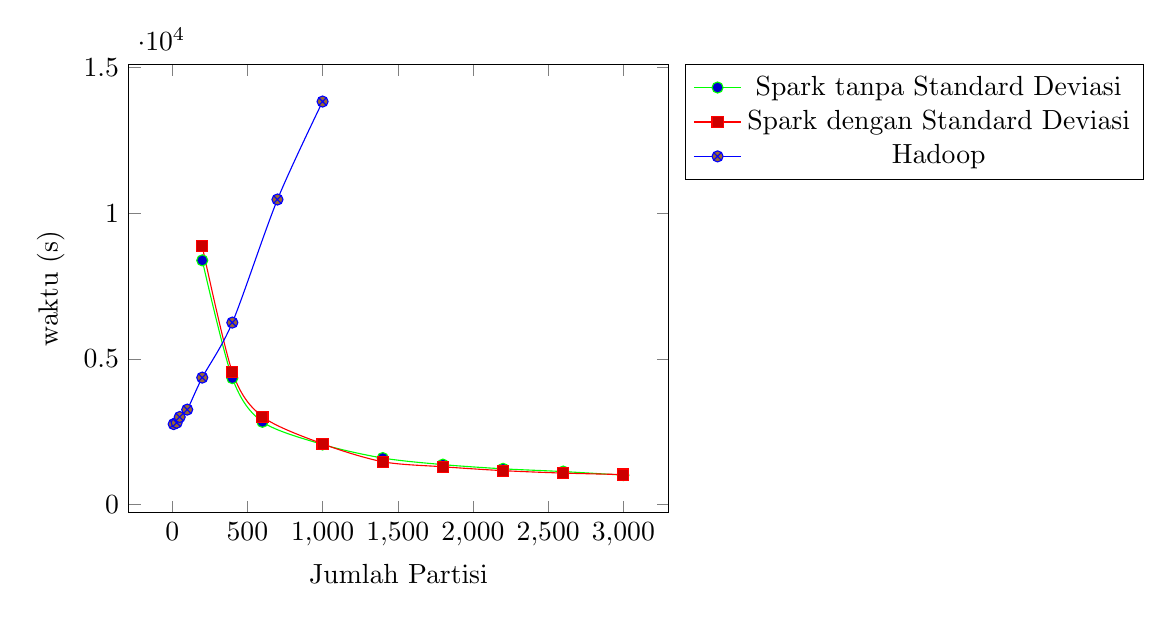
\begin{tikzpicture}[scale=\scl]
		\begin{axis}[\ymin,\ymax,xlabel= Jumlah Partisi,ylabel= waktu (s), xticklabel style={/pgf/number format/.cd, fixed,fixed zerofill, precision=0},legend pos = outer north east]
		
		\addlegendentry{Spark tanpa Standard Deviasi}
		\addplot+[smooth][color=green] coordinates { (200,8386) (400,4342) (600,2841) (1000,2065) (1400,1598) (1800,1372) (2200,1228) (2600,1133) (3000,1010)};
		\addlegendentry{Spark dengan Standard Deviasi}
		\addplot+[smooth][color=red] coordinates {(200,8866) (400,4553) (600,3021) (1000,2084) (1400,1471) (1800,1298) (2200,1165) (2600,1081) (3000,1031)};
		\addlegendentry{Hadoop}
		\addplot+[smooth][color=blue] coordinates {(10,2763) (30,2811) (50,3007) (100,3261) (200,4360) (400,6249) (700,10476) (1000,13839)};

		

		\leg
		\end{axis}
		\end{tikzpicture}
		\caption[Hasil percobaan partisi Spark dan Hadoop 20GB]{Hasil percobaan partisi Spark dan Hadoop 20GB}
		\label{fig:percobaan2}
	\end{figure}
\end{minipage}\\




%%%%%%%%%%%%%%%%MAX OBJ 50




%%%%%%%%%%%%%%%%%%%%%%%%%%%%%%%%%%%MAX OBJ 50 15 GB


Pada percobaan ini akan dilihat waktu eksekusi Spark dan Hadoop berdasarkan jumlah partisi yang optimal. Percobaan ini akan menggunakan 1 komputer sebagai komputer \textit{master} dan 10 komputer lainya sebagai \textit{worker} dengan setiap \textit{worker} munggunakan 1 core. Ukuran data yang digunakan adalah 15 GB. Metode yang dingunakan adalah metode \textit{single linkage}, dengan nilai \textit{cut-off distance} adalah 0,8 dan jumlah objek maksimum untuk setiap \textit{dendrogram} adalah 50. Tabel (~\ref{tab:spark11} dan Tabel (~\ref{tab:spark12}) berikut adalah hasil dari eksperimen:





\begin{table}[H] 
	\centering 
	\caption{Percobaan Jumlah Partisi Hadoop dengan Ukuran Data 15 GB}
	\label{tab:spark10}
	\begin{tabular}{|p{3cm}|p{3cm}|p{4cm}|p{4cm}|}
\hline
Ukuran Data (GB) & Jumlah Partisi &  Waktu Eksekusi Hadoop (detik) & Hasil Reduksi Hadoop (GB)\\
\hline
15 & 10 & 4273  & 4.2 \\
\hline
15 & 30 & 4319  & 4.2 \\
\hline
15 & 50 & 4464  & 4.2  \\
\hline


\hline

	\end{tabular} 
\end{table}



\def\scl{1}

\def\leg{} 
\def\std{none}
\def\ymin{}
\def\ymax{}

\begin{minipage}[c]{0.9\textwidth}
	\begin{figure}[H]
		\centering
		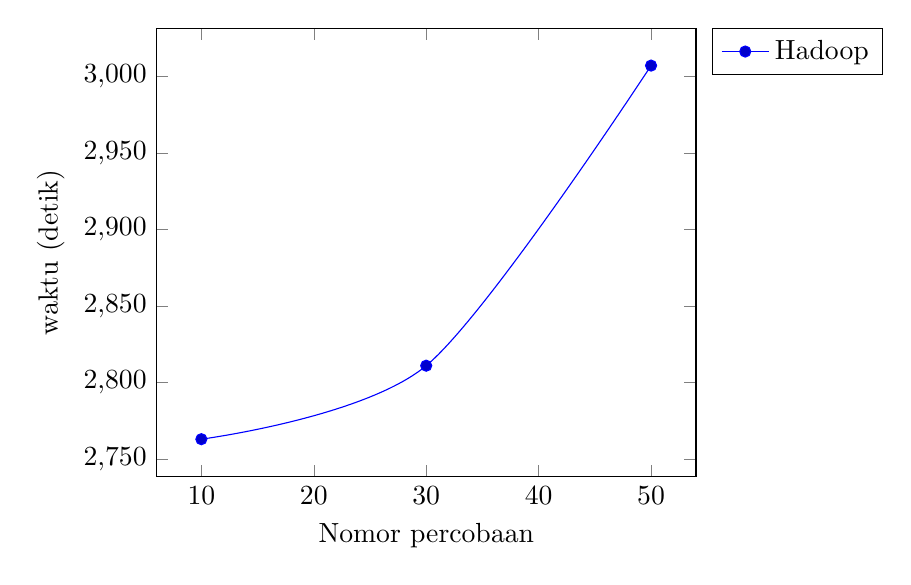
\begin{tikzpicture}[scale=\scl]
		\begin{axis}[\ymin,\ymax,xlabel= Nomor percobaan,ylabel= waktu (detik), xticklabel style={/pgf/number format/.cd, fixed,fixed zerofill, precision=0},legend pos = outer north east]

		\addlegendentry{Hadoop}
		\addplot+[smooth][color=blue] coordinates {(10,2763) (30,2811) (50,3007) };

		

		\leg
		\end{axis}
		\end{tikzpicture}
		\caption[Hasil percobaan partisi Spark dan Hadoop 20GB]{Hasil percobaan partisi Spark dan Hadoop 20GB}
		\label{fig:percobaan2}
	\end{figure}
\end{minipage}\\




\begin{table}[H] 
	\centering 
	\caption{Percobaan Jumlah Partisi Hadoop dengan Ukuran Data 20}
	\label{tab:spark9}
	\begin{tabular}{|p{1cm}|p{1cm}|p{3cm}|p{3cm}|p{3cm}|p{3cm}|}
\hline
Ukuran Data (GB) & Jumlah Partisi &  Waktu Ekseuksi Spark Tanpa Standard Deviasi (detik) & Waktu Eksekusi Spark (detik) & Hasil Reduksi Spark Tanpa Standard Deviasi (GB) & Hasil Reduksi Spark (GB)  \\ 
\hline
20 & 1200 & 1135  & 1043  & 4.2 & 5.2 \\
\hline
20 & 1500 & 911  & 961  & 4.2 & 5.2 \\
\hline
20 & 1800 & 883  & 884  &  4.2 & 5.2 \\
\hline

\hline

	\end{tabular} 
\end{table}



\def\scl{1}

\def\leg{} 
\def\std{none}
\def\ymin{}
\def\ymax{}

\begin{minipage}[c]{0.9\textwidth}
	\begin{figure}[H]
		\centering
		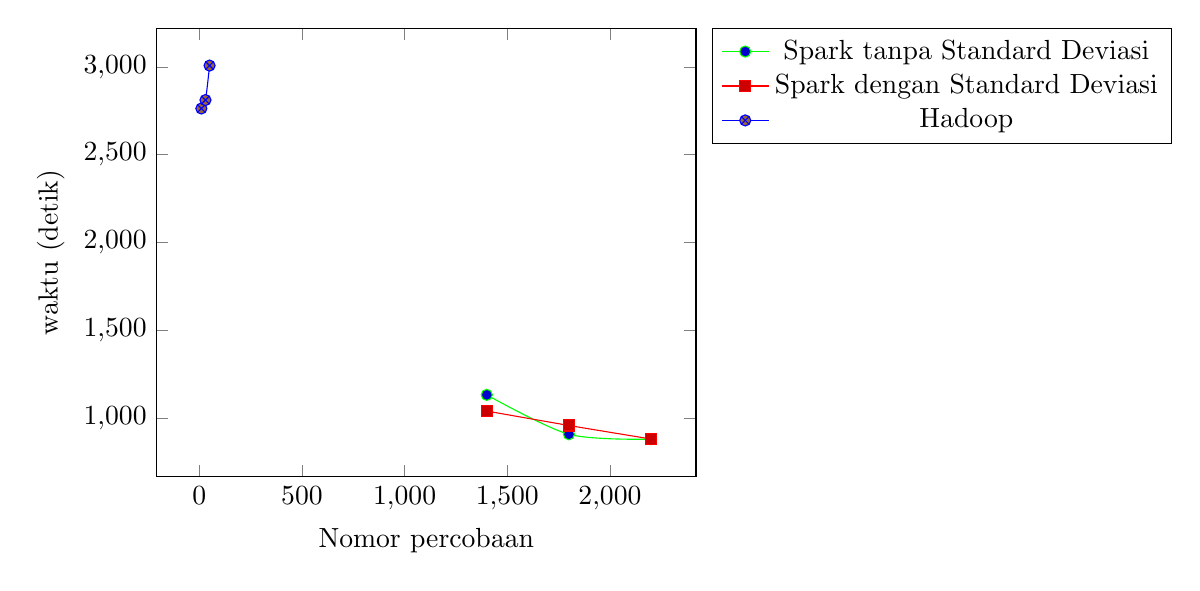
\begin{tikzpicture}[scale=\scl]
		\begin{axis}[\ymin,\ymax,xlabel= Nomor percobaan,ylabel= waktu (detik), xticklabel style={/pgf/number format/.cd, fixed,fixed zerofill, precision=0},legend pos = outer north east]
		
		\addlegendentry{Spark tanpa Standard Deviasi}
		\addplot+[smooth][color=green] coordinates { (1400,1135) (1800,911) (2200,883)};
		\addlegendentry{Spark dengan Standard Deviasi}
		\addplot+[smooth][color=red] coordinates { (1400,1043) (1800,961) (2200,884)};
		\addlegendentry{Hadoop}
		\addplot+[smooth][color=blue] coordinates {(10,2763) (30,2811) (50,3007) };

		

		\leg
		\end{axis}
		\end{tikzpicture}
		\caption[Hasil percobaan partisi Spark dan Hadoop 20GB]{Hasil percobaan partisi Spark dan Hadoop 20GB}
		\label{fig:percobaan2}
	\end{figure}
\end{minipage}\\




%%%%%%%%%%%%%%%%%%%%%% MAX OBJ 50 20GB


Pada percobaan ini akan dilihat waktu eksekusi Spark dan Hadoop dengan nilai objek maksimum pada sebuah dendrogram adalah 50. Berdasarkan percobaan sebelumnya akan digunakan jumlah partisi yang optimal untuk keduanya. Percobaan ini akan menggunakan 1 komputer sebagai komputer \textit{master} dan 10 komputer lainya sebagai \textit{worker} dengan setiap \textit{worker} munggunakan 1 core. Ukuran data yang digunakan adalah 20 GB. Metode yang dingunakan adalah metode \textit{single linkage}, dengan nilai \textit{cut-off distance} adalah 0,8 dan jumlah objek maksimum untuk setiap \textit{dendrogram} adalah 50. Tabel (~\ref{tab:spark11} dan Tabel (~\ref{tab:spark12}) berikut adalah hasil dari eksperimen:





\begin{table}[H] 
	\centering 
	\caption{Percobaan Jumlah Partisi Hadoop dengan Ukuran Data 20 GB}
	\label{tab:spark10}
	\begin{tabular}{|p{3cm}|p{3cm}|p{4cm}|p{4cm}|}
\hline
Ukuran Data (GB) & Jumlah Partisi &  Waktu Eksekusi Hadoop (detik) & Hasil Reduksi Hadoop (GB)\\
\hline
20 & 10 & 5462  & 5.6 \\
\hline
20 & 30 & 5771  & 5.6 \\
\hline
20 & 50 & 6840  & 5.6  \\
\hline


\hline

	\end{tabular} 
\end{table}



\def\scl{1}

\def\leg{} 
\def\std{none}
\def\ymin{}
\def\ymax{}

\begin{minipage}[c]{0.9\textwidth}
	\begin{figure}[H]
		\centering
		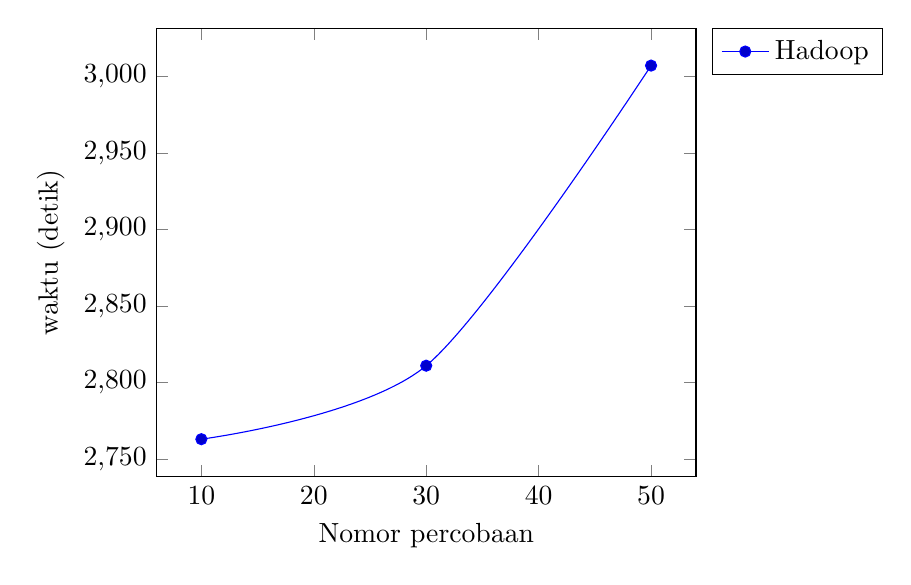
\begin{tikzpicture}[scale=\scl]
		\begin{axis}[\ymin,\ymax,xlabel= Nomor percobaan,ylabel= waktu (detik), xticklabel style={/pgf/number format/.cd, fixed,fixed zerofill, precision=0},legend pos = outer north east]

		\addlegendentry{Hadoop}
		\addplot+[smooth][color=blue] coordinates {(10,2763) (30,2811) (50,3007) };

		

		\leg
		\end{axis}
		\end{tikzpicture}
		\caption[Hasil percobaan partisi Spark dan Hadoop 20GB]{Hasil percobaan partisi Spark dan Hadoop 20GB}
		\label{fig:percobaan2}
	\end{figure}
\end{minipage}\\




\begin{table}[H] 
	\centering 
	\caption{Percobaan Jumlah Partisi Hadoop dengan Ukuran Data 20}
	\label{tab:spark9}
	\begin{tabular}{|p{1cm}|p{1cm}|p{3cm}|p{3cm}|p{3cm}|p{3cm}|}
\hline
Ukuran Data (GB) & Jumlah Partisi &  Waktu Ekseuksi Spark Tanpa Standard Deviasi (detik) & Waktu Eksekusi Spark (detik) & Hasil Reduksi Spark Tanpa Standard Deviasi (GB) & Hasil Reduksi Spark (GB)  \\ 
\hline
20 & 1400 & 1135  & 1043  & 5.6 & 6.9 \\
\hline
20 & 1800 & 911  & 961  & 5.6 & 6.9 \\
\hline
20 & 2200 & 883  & 884  &  5.6 & 6.9 \\
\hline

\hline

	\end{tabular} 
\end{table}


\def\scl{1}

\def\leg{} 
\def\std{none}
\def\ymin{}
\def\ymax{}

\begin{minipage}[c]{0.9\textwidth}
	\begin{figure}[H]
		\centering
		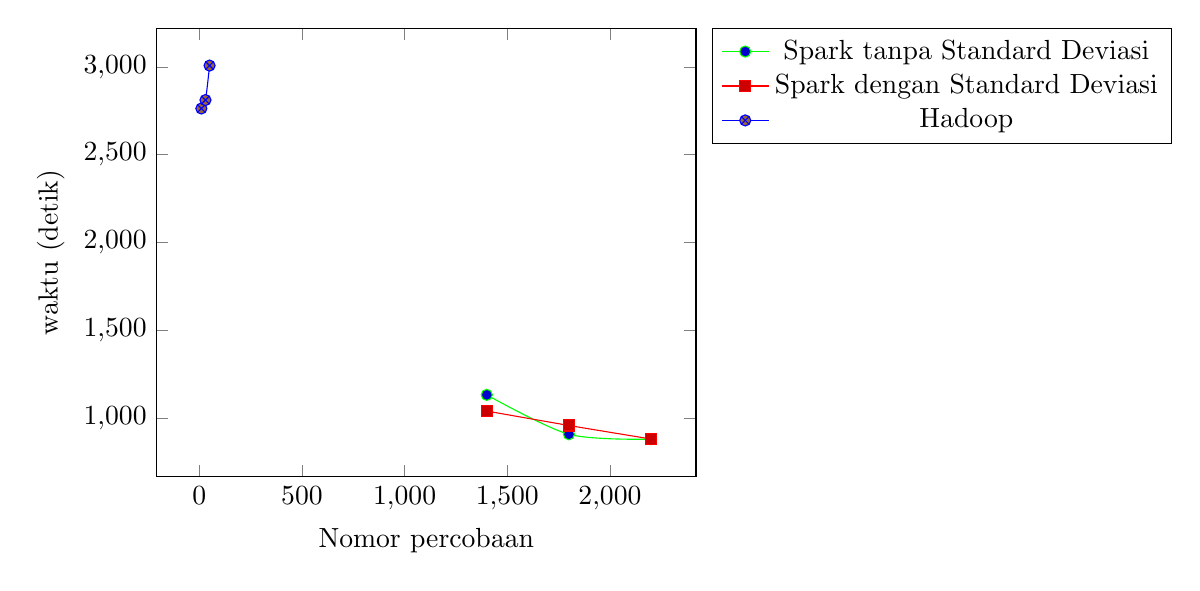
\begin{tikzpicture}[scale=\scl]
		\begin{axis}[\ymin,\ymax,xlabel= Nomor percobaan,ylabel= waktu (detik), xticklabel style={/pgf/number format/.cd, fixed,fixed zerofill, precision=0},legend pos = outer north east]
		
		\addlegendentry{Spark tanpa Standard Deviasi}
		\addplot+[smooth][color=green] coordinates { (1400,1135) (1800,911) (2200,883)};
		\addlegendentry{Spark dengan Standard Deviasi}
		\addplot+[smooth][color=red] coordinates { (1400,1043) (1800,961) (2200,884)};
		\addlegendentry{Hadoop}
		\addplot+[smooth][color=blue] coordinates {(10,2763) (30,2811) (50,3007) };

		

		\leg
		\end{axis}
		\end{tikzpicture}
		\caption[Hasil percobaan partisi Spark dan Hadoop 20GB]{Hasil percobaan partisi Spark dan Hadoop 20GB}
		\label{fig:percobaan2}
	\end{figure}
\end{minipage}\\

